\documentclass{standalone}
\usepackage{tikz}
\usetikzlibrary{patterns, positioning}


\begin{document}
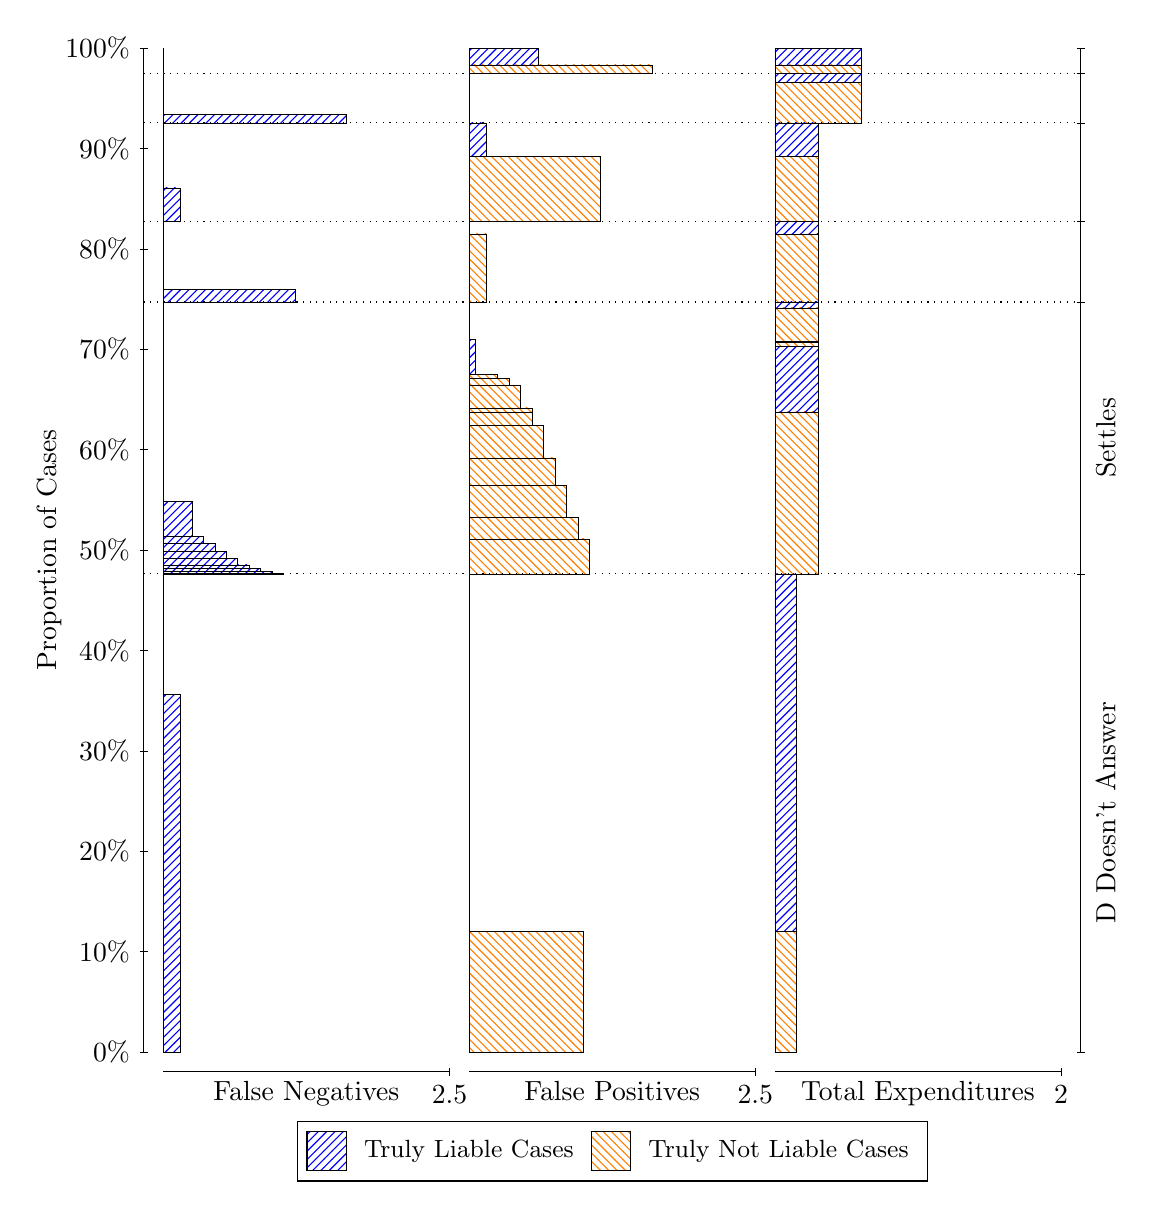
\begin{tikzpicture}
\draw[black, very thin] (1.5,1.75) -- (1.5,14.5);
\node[rotate=90, text=black, anchor=center] at (0.3, 8.125) {Proportion of Cases};
\draw[black, very thin] (1.45,1.75) -- (1.55,1.75);
\node[text=black, anchor=east] at (1.45, 1.75) {0\%};
\draw[black, very thin] (1.45,3.025) -- (1.55,3.025);
\node[text=black, anchor=east] at (1.45, 3.025) {10\%};
\draw[black, very thin] (1.45,4.3) -- (1.55,4.3);
\node[text=black, anchor=east] at (1.45, 4.3) {20\%};
\draw[black, very thin] (1.45,5.575) -- (1.55,5.575);
\node[text=black, anchor=east] at (1.45, 5.575) {30\%};
\draw[black, very thin] (1.45,6.85) -- (1.55,6.85);
\node[text=black, anchor=east] at (1.45, 6.85) {40\%};
\draw[black, very thin] (1.45,8.125) -- (1.55,8.125);
\node[text=black, anchor=east] at (1.45, 8.125) {50\%};
\draw[black, very thin] (1.45,9.4) -- (1.55,9.4);
\node[text=black, anchor=east] at (1.45, 9.4) {60\%};
\draw[black, very thin] (1.45,10.675) -- (1.55,10.675);
\node[text=black, anchor=east] at (1.45, 10.675) {70\%};
\draw[black, very thin] (1.45,11.95) -- (1.55,11.95);
\node[text=black, anchor=east] at (1.45, 11.95) {80\%};
\draw[black, very thin] (1.45,13.225) -- (1.55,13.225);
\node[text=black, anchor=east] at (1.45, 13.225) {90\%};
\draw[black, very thin] (1.45,14.5) -- (1.55,14.5);
\node[text=black, anchor=east] at (1.45, 14.5) {100\%};

\draw[black, very thin] (13.4,1.75) -- (13.4,14.5);
\draw[black, very thin] (13.35,1.75) -- (13.45,1.75);
\node[anchor=west] at (13.35, 1.75) {};
\draw[black, very thin] (13.35,7.8229) -- (13.45,7.8229);
\node[anchor=west] at (13.35, 7.8229) {};
\draw[black, very thin] (13.35,11.275) -- (13.45,11.275);
\node[anchor=west] at (13.35, 11.275) {};
\draw[black, very thin] (13.35,12.296) -- (13.45,12.296);
\node[anchor=west] at (13.35, 12.296) {};
\draw[black, very thin] (13.35,13.549) -- (13.45,13.549);
\node[anchor=west] at (13.35, 13.549) {};
\draw[black, very thin] (13.35,14.178) -- (13.45,14.178);
\node[anchor=west] at (13.35, 14.178) {};
\draw[black, very thin] (13.35,14.5) -- (13.45,14.5);
\node[anchor=west] at (13.35, 14.5) {};

\draw[black, very thin, pattern color=blue, pattern=north east lines] (1.75,1.75) rectangle (1.968,6.2927);
\draw[black, very thin, pattern color=orange, pattern=north west lines] (1.75,6.2927) rectangle (1.75,7.8229);
\draw[black, very thin, pattern color=blue, pattern=north east lines] (1.75,7.8229) rectangle (3.276,7.8328);
\draw[black, very thin, pattern color=blue, pattern=north east lines] (1.75,7.8328) rectangle (3.1307,7.8489);
\draw[black, very thin, pattern color=blue, pattern=north east lines] (1.75,7.8489) rectangle (2.9853,7.8944);
\draw[black, very thin, pattern color=blue, pattern=north east lines] (1.75,7.8944) rectangle (2.84,7.9346);
\draw[black, very thin, pattern color=blue, pattern=north east lines] (1.75,7.9346) rectangle (2.6947,8.0214);
\draw[black, very thin, pattern color=blue, pattern=north east lines] (1.75,8.0214) rectangle (2.5493,8.1068);
\draw[black, very thin, pattern color=blue, pattern=north east lines] (1.75,8.1068) rectangle (2.404,8.2135);
\draw[black, very thin, pattern color=blue, pattern=north east lines] (1.75,8.2135) rectangle (2.2587,8.2968);
\draw[black, very thin, pattern color=blue, pattern=north east lines] (1.75,8.2968) rectangle (2.1133,8.7449);
\draw[black, very thin, pattern color=orange, pattern=north west lines] (1.75,8.7449) rectangle (1.75,11.275);
\draw[black, very thin, pattern color=blue, pattern=north east lines] (1.75,11.275) rectangle (3.4213,11.433);
\draw[black, very thin, pattern color=orange, pattern=north west lines] (1.75,11.433) rectangle (1.75,12.296);
\draw[black, very thin, pattern color=blue, pattern=north east lines] (1.75,12.296) rectangle (1.968,12.725);
\draw[black, very thin, pattern color=orange, pattern=north west lines] (1.75,12.725) rectangle (1.75,13.549);
\draw[black, very thin, pattern color=blue, pattern=north east lines] (1.75,13.549) rectangle (4.0753,13.66);
\draw[black, very thin, pattern color=orange, pattern=north west lines] (1.75,13.66) rectangle (1.75,14.178);
\draw[black, very thin, pattern color=orange, pattern=north west lines] (1.75,14.178) rectangle (1.75,14.287);
\draw[black, very thin, pattern color=blue, pattern=north east lines] (1.75,14.287) rectangle (1.75,14.5);
\draw[black, very thin, pattern color=orange, pattern=north west lines] (5.6333,1.75) rectangle (7.0867,3.2802);
\draw[black, very thin, pattern color=blue, pattern=north east lines] (5.6333,3.2802) rectangle (5.6333,7.8229);
\draw[black, very thin, pattern color=orange, pattern=north west lines] (5.6333,7.8229) rectangle (7.1593,8.2651);
\draw[black, very thin, pattern color=orange, pattern=north west lines] (5.6333,8.2651) rectangle (7.014,8.5417);
\draw[black, very thin, pattern color=orange, pattern=north west lines] (5.6333,8.5417) rectangle (6.8687,8.9483);
\draw[black, very thin, pattern color=orange, pattern=north west lines] (5.6333,8.9483) rectangle (6.7233,9.2956);
\draw[black, very thin, pattern color=orange, pattern=north west lines] (5.6333,9.2956) rectangle (6.578,9.7069);
\draw[black, very thin, pattern color=orange, pattern=north west lines] (5.6333,9.7069) rectangle (6.4327,9.878);
\draw[black, very thin, pattern color=orange, pattern=north west lines] (5.6333,9.878) rectangle (6.4327,9.929);
\draw[black, very thin, pattern color=orange, pattern=north west lines] (5.6333,9.929) rectangle (6.2873,10.215);
\draw[black, very thin, pattern color=orange, pattern=north west lines] (5.6333,10.215) rectangle (6.142,10.303);
\draw[black, very thin, pattern color=orange, pattern=north west lines] (5.6333,10.303) rectangle (5.9967,10.353);
\draw[black, very thin, pattern color=blue, pattern=north east lines] (5.6333,10.353) rectangle (5.706,10.801);
\draw[black, very thin, pattern color=blue, pattern=north east lines] (5.6333,10.801) rectangle (5.6333,11.275);
\draw[black, very thin, pattern color=orange, pattern=north west lines] (5.6333,11.275) rectangle (5.8513,12.139);
\draw[black, very thin, pattern color=blue, pattern=north east lines] (5.6333,12.139) rectangle (5.6333,12.296);
\draw[black, very thin, pattern color=orange, pattern=north west lines] (5.6333,12.296) rectangle (7.3047,13.121);
\draw[black, very thin, pattern color=blue, pattern=north east lines] (5.6333,13.121) rectangle (5.8513,13.549);
\draw[black, very thin, pattern color=orange, pattern=north west lines] (5.6333,13.549) rectangle (5.6333,14.067);
\draw[black, very thin, pattern color=blue, pattern=north east lines] (5.6333,14.067) rectangle (5.6333,14.178);
\draw[black, very thin, pattern color=orange, pattern=north west lines] (5.6333,14.178) rectangle (7.9587,14.287);
\draw[black, very thin, pattern color=blue, pattern=north east lines] (5.6333,14.287) rectangle (6.5053,14.5);
\draw[black, very thin, pattern color=orange, pattern=north west lines] (9.5167,1.75) rectangle (9.7892,3.2802);
\draw[black, very thin, pattern color=blue, pattern=north east lines] (9.5167,3.2802) rectangle (9.7892,7.8229);
\draw[black, very thin, pattern color=orange, pattern=north west lines] (9.5167,7.8229) rectangle (10.062,9.878);
\draw[black, very thin, pattern color=blue, pattern=north east lines] (9.5167,9.878) rectangle (10.062,10.714);
\draw[black, very thin, pattern color=orange, pattern=north west lines] (9.5167,10.714) rectangle (10.062,10.764);
\draw[black, very thin, pattern color=blue, pattern=north east lines] (9.5167,10.764) rectangle (10.062,10.774);
\draw[black, very thin, pattern color=orange, pattern=north west lines] (9.5167,10.774) rectangle (10.062,11.199);
\draw[black, very thin, pattern color=blue, pattern=north east lines] (9.5167,11.199) rectangle (10.062,11.275);
\draw[black, very thin, pattern color=orange, pattern=north west lines] (9.5167,11.275) rectangle (10.062,12.139);
\draw[black, very thin, pattern color=blue, pattern=north east lines] (9.5167,12.139) rectangle (10.062,12.296);
\draw[black, very thin, pattern color=orange, pattern=north west lines] (9.5167,12.296) rectangle (10.062,13.121);
\draw[black, very thin, pattern color=blue, pattern=north east lines] (9.5167,13.121) rectangle (10.062,13.549);
\draw[black, very thin, pattern color=orange, pattern=north west lines] (9.5167,13.549) rectangle (10.607,14.067);
\draw[black, very thin, pattern color=blue, pattern=north east lines] (9.5167,14.067) rectangle (10.607,14.178);
\draw[black, very thin, pattern color=orange, pattern=north west lines] (9.5167,14.178) rectangle (10.607,14.287);
\draw[black, very thin, pattern color=blue, pattern=north east lines] (9.5167,14.287) rectangle (10.607,14.5);
\draw[black, dotted] (1.5,7.8229) -- (13.4,7.8229);
\draw[black, dotted] (1.5,11.275) -- (13.4,11.275);
\draw[black, dotted] (1.5,12.296) -- (13.4,12.296);
\draw[black, dotted] (1.5,13.549) -- (13.4,13.549);
\draw[black, dotted] (1.5,14.178) -- (13.4,14.178);
\draw[black, very thin] (1.75,1.5) -- (5.3833,1.5);
\node[text=black, anchor=north] at (3.5667, 1.5) {False Negatives};
\draw[black, very thin] (5.3833,1.45) -- (5.3833,1.55);
\node[text=black, anchor=north] at (5.3833, 1.45) {2.5};

\draw[black, very thin] (5.6333,1.5) -- (9.2667,1.5);
\node[text=black, anchor=north] at (7.45, 1.5) {False Positives};
\draw[black, very thin] (9.2667,1.45) -- (9.2667,1.55);
\node[text=black, anchor=north] at (9.2667, 1.45) {2.5};

\draw[black, very thin] (9.5167,1.5) -- (13.15,1.5);
\node[text=black, anchor=north] at (11.333, 1.5) {Total Expenditures};
\draw[black, very thin] (13.15,1.45) -- (13.15,1.55);
\node[text=black, anchor=north] at (13.15, 1.45) {2};

\node[text=black, centered, rotate=90] at (13.72, 4.7864) {D Doesn't Answer};
\node[text=black, centered, rotate=90] at (13.72, 9.5489) {Settles};





\draw (7.449999999999999,1.5) node[draw=none] (baseCoordinate) {};
\begin{scope}[align=center]
        \matrix[scale=0.5, draw=black, below=0.5cm of baseCoordinate, nodes={draw}, column sep=0.1cm]{
            \node[rectangle, draw, minimum width=0.5cm, minimum height=0.5cm, pattern color=blue, pattern=north east lines] {}; &
            \node[draw=none, font=\small, text=black] (B) {Truly Liable Cases}; &
            \node[rectangle, draw, minimum width=0.5cm, minimum height=0.5cm, pattern color=orange, pattern=north west lines] {}; &
            \node[draw=none, font=\small, text=black] (B) {Truly Not Liable Cases}; \\
            };
\end{scope}

\end{tikzpicture}
\end{document}